\section[Bleek\& Lloyd collection]{Bleek and Lloyd collection}\index{Bleek and Lloyd}
\label{sec:case-studies:bleek-and-lloyd}

\begin{figure}
 %\begin{center}
  \centering
  \framebox[\textwidth]{%
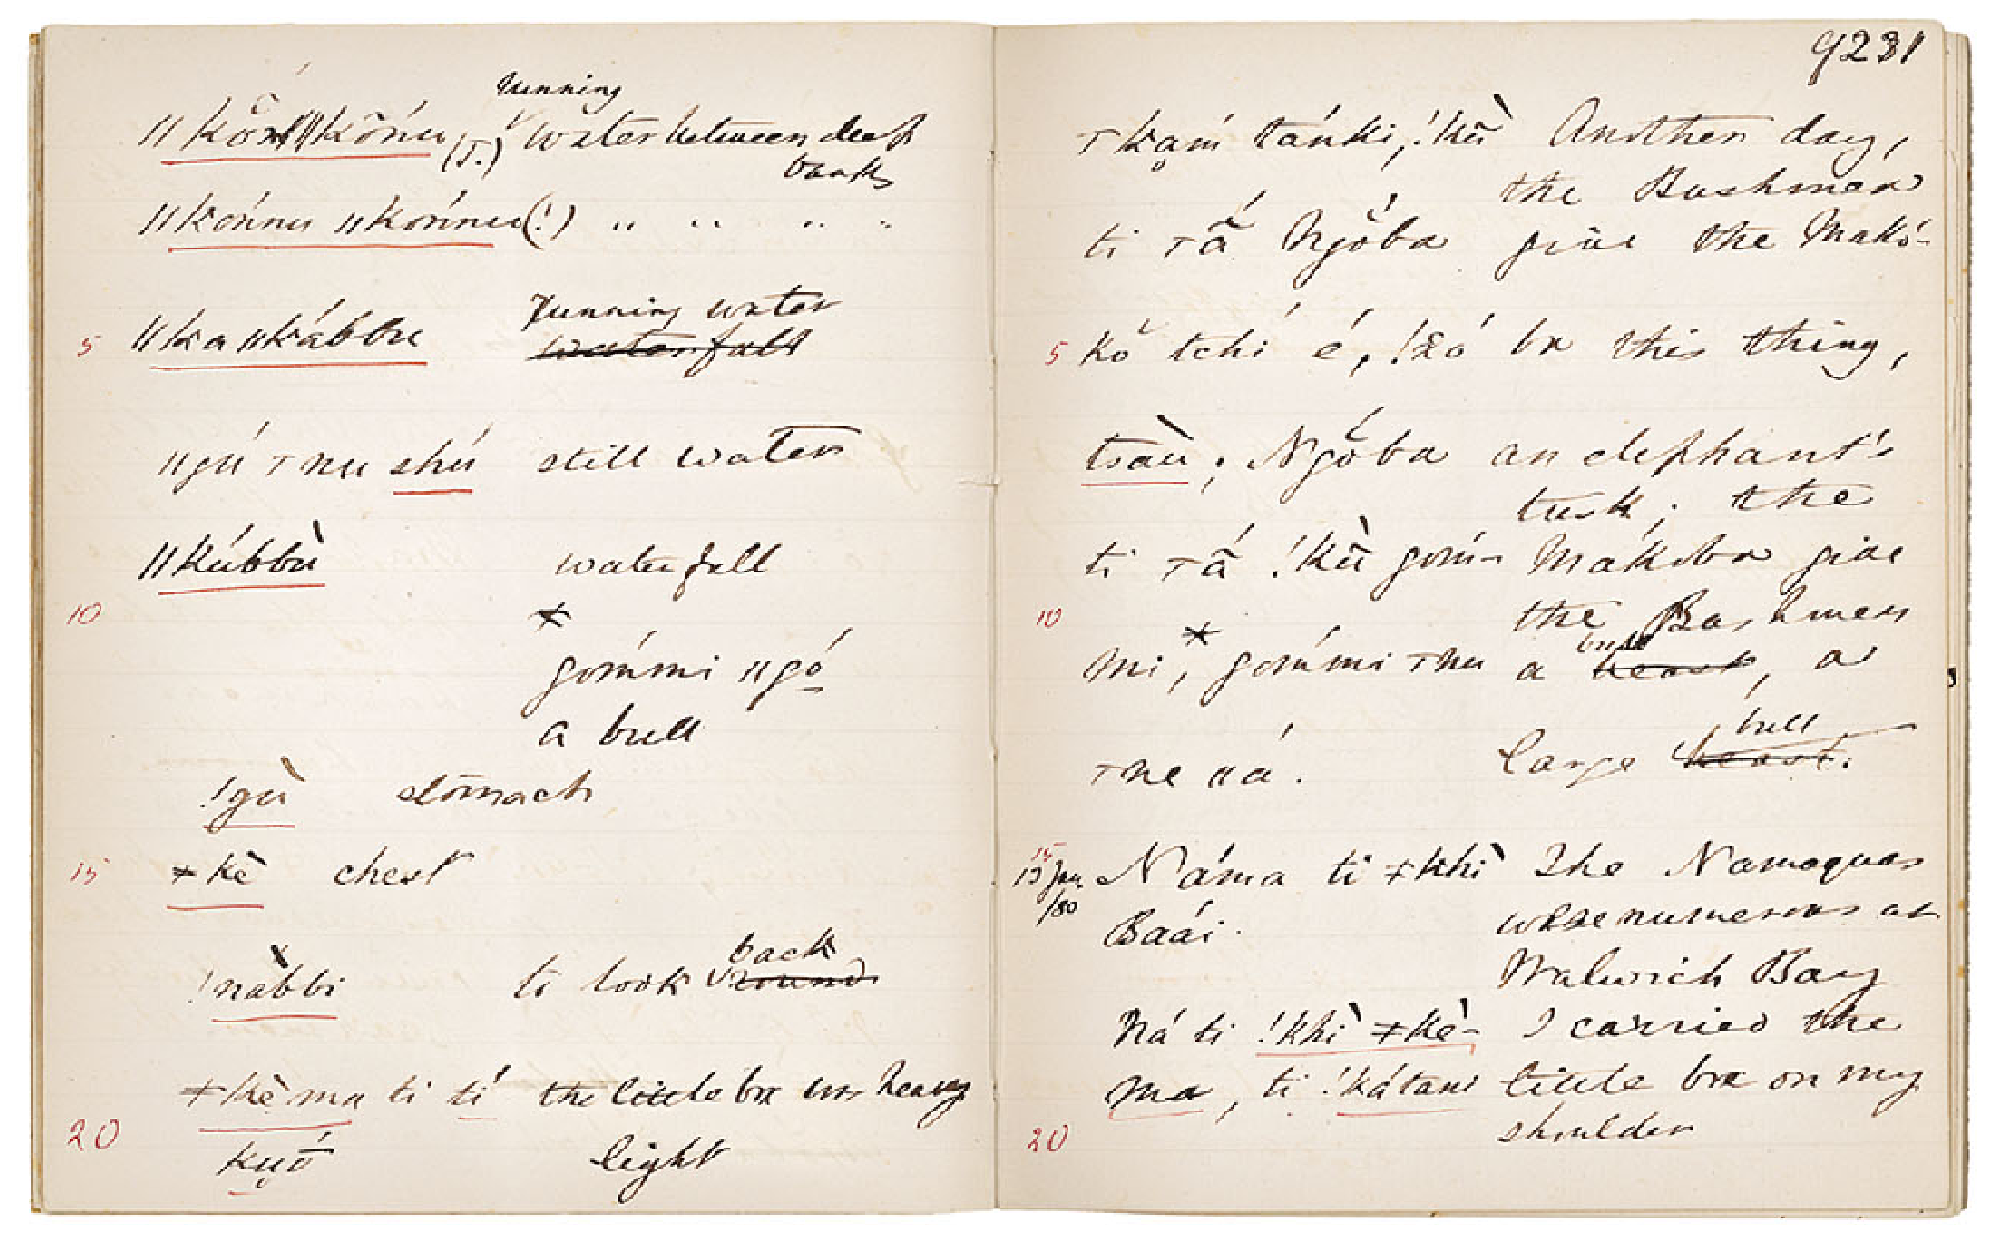
\includegraphics[width=0.95\textwidth]{chapter06/figures/case-studies.bleek-and-lloyd.A2_1_112_09231.eps}%
}%
\caption[Screenshot showing a sample page from Bleek\& Lloyd collection]{Screenshot showing a sample page from the ``Posts and trading'' story in the Lucy Lloyd !Kun notebooks}
\label{fig:case-studies:bleek-and-lloyd:brief-history:case-studies.bleek-and-lloyd.A2_1_112_09231}
% \end{center}
\end{figure}

%%%%%\subsection[Bushman folklore]{Bushman folklore}
%%%%%\label{sec:case-studies:bleek-and-lloyd:bushman-folklore}
%%%%%\subsection[Brief history]{Brief history}
\subsection[Overview]{Overview}
\label{sec:case-studies:bleek-and-lloyd:brief-history}

The Bleek and Lloyd collection \citep{Skotnes2007} is a 19th century compilation of notebooks and drawings comprising of linguistic and ethnographic work of Lucy Lloyd and Wilhelm Bleek on the life of the \textbar Xam\index{Xam} and !Kun\index{Kun} Bushman people of Southern Africa. In 2003, the Lucy Lloyd Archive and Research centre at the University of Cape Town embarked on a large scale digitisation project and all the artifacts are in the process of being scanned and corresponding representation information generated. Table~\ref{tab:case-studies:overview:lloydbleek-database-collection} shows the current composition of the digitised objects and Figure~\ref{fig:case-studies:bleek-and-lloyd:brief-history:case-studies.bleek-and-lloyd.A2_1_112_09231} shows a sample page from one of the digitised notebooks.

%\subsection{Non-Functional Requirements}
%\label{sec:design-implementation:design-process:non-functional-requirements}
%http://upload.wikimedia.org/wikipedia/commons/2/2b/Data_modeling_context.svg

%\begin{comment}
% PLEASE SEE PAGE 51---overview of strategies table
%
%http://jeffrey.famvdhoeven.nl/Researchtask%20IBM%20TU%20Delft%20-%20J.R.%20van%
%20der%20Hoeven.pdf
%\end{comment}

%Nice table outline here
%(\url{
%http://www.slideshare.net/henry.muccini/software-architecture-design-decisions}
%)
%Questions
%Options
%criteria

\tablespacing
%%%%%\begin{longtable}{p{0.4\linewidth} p{0.5\linewidth}}
\begin{longtable}{
>{\arraybackslash}p{0.30\linewidth}|
>{\arraybackslash}p{0.60\linewidth}}

\caption{Bleek\& Lloyd collection profile}
\label{tab:case-studies:overview:lloydbleek-database-collection} \\

 %%%%%%\toprule
 %%%%%\textbf{} & \textbf{}\\
 %%%%%\cline{1-2}
 \endfirsthead

 \caption[]{(continued)}\\
 %%%%%%\toprule
 %%%%%\textbf{} & \textbf{}\\
 %%%%%\cline{1-2}
 \endhead

 % Page footer
 \midrule
 \multicolumn{2}{r}{(Continued on next page)} \\
 \endfoot

 % Last page footer
 %%%%%%\bottomrule
 \endlastfoot

 %%%%%{} &
 %%%%%{} \\
 %%%%%\cline{1-2}
 %\cmidrule[0.1pt](l{0.5em}r{0.5em}){1-2}

 {\textbf{Collection theme}} &
 {Historical artifacts; museum objects}\\

 \cline{1-2}
 %\cmidrule[0.1pt](l{0.5em}r{0.5em}){1-2}

 {\textbf{Media types}} &
 {Digitised}\\

 \cline{1-2}
 %\cmidrule[0.1pt](l{0.5em}r{0.5em}){1-2}

 {\textbf{Collection size}} &
 {6.2GB}\\

 \cline{1-2}
 %\cmidrule[0.1pt](l{0.5em}r{0.5em}){1-2}

 {\textbf{Content type}} &
 {image/jpeg}\\

 \cline{1-2}
 %\cmidrule[0.1pt](l{0.5em}r{0.5em}){1-2}

 {\textbf{Number of collections}} &
 {\num{6}}\\

 \cline{1-2}
 %\cmidrule[0.1pt](l{0.5em}r{0.5em}){1-2}

 {\textbf{Number of objects}} &
 {\num{18924}}\\

 %%%%%\cline{1-2}
 %\cmidrule[0.1pt](l{0.5em}r{0.5em}){1-2}

 \end{longtable}

\bodyspacing

\subsection{Object storage}
\label{sec:case-studies:bleek-and-lloyd:implementation}

\tablespacing
%%%%%\begin{longtable}{p{0.3\linewidth} p{0.6\linewidth}}
\begin{longtable}{
>{\arraybackslash}p{0.20\linewidth}|
>{\arraybackslash}p{0.25\linewidth}|
>{\arraybackslash}p{0.45\linewidth}}

\caption{Bleek\& Lloyd repository item classification}
\label{tab:case-studies:bleek-and-lloyd:object-organisation} \\

 %%%%%\toprule
 %%%%%\hline
 \textbf{Item} & 
 \textbf{Object Type} & 
 \textbf{Comments}\\
 %%%%%\midrule
 %%%%%\hline
 \cline{1-3}
 \endfirsthead

 \caption[]{(continued)}\\
 %%%%%\toprule
 %%%%%\hline
 \textbf{Item Type} & 
 \textbf{Object Type} & 
 \textbf{Comments}\\
 %%%%%\midrule
 %%%%%\hline
 \cline{1-3}
 \endhead

 % Page footer
 %%%%%\midrule
 %%%%%\hline
 \multicolumn{3}{r}{(Continued on next page)} \\
 \endfoot

 % Last page footer
 %%%%%\bottomrule
 \endlastfoot

 {\textbf{Notebook}}&
 {Container object} &
 {Author compilation of books} \\

 %%%%%\cmidrule[0.1pt](l{0.5em}r{0.5em}){1-2}
 \cline{1-3}

 {\textbf{Book}} &
 {Container object} &
 {Compilation of digitised pages} \\

 %%%%%\cmidrule[0.1pt](l{0.5em}r{0.5em}){1-2}
 \cline{1-3}

 {\textbf{Story}} &
 {Content object} &
 {Content object without bitsreams} \\

 %%%%%\cmidrule[0.1pt](l{0.5em}r{0.5em}){1-2}
 \cline{1-3}

 {\textbf{Page}} &
 {Content object} &
 {Digitised page} \\

 %%%%%\cmidrule[0.1pt](l{0.5em}r{0.5em}){1-2}
 %%%%%\cline{1-3}

 \end{longtable}

\bodyspacing

Table~\ref{tab:case-studies:bleek-and-lloyd:object-organisation} shows the object composition of the collection and Figure~\ref{fig:case-studies:bleek-and-lloyd:object-storage:object-relationships} shows the relationships among the objects.

\begin{figure}
 \centering
 \framebox[\textwidth]{
 % Generated with LaTeXDraw 2.0.8
% Sun Mar 03 17:46:51 SAST 2013
% \usepackage[usenames,dvipsnames]{pstricks}
% \usepackage{epsfig}
% \usepackage{pst-grad} % For gradients
% \usepackage{pst-plot} % For axes
\scalebox{1} % Change this value to rescale the drawing.
{
\begin{pspicture}(0,-4.24)(11.44,4.08)
\definecolor{color126b}{rgb}{0.7176470588235294,0.8862745098039215,0.9411764705882353}
\psline[linewidth=0.06cm](9.34,-2.96)(4.72,-0.64)
\psline[linewidth=0.06cm](1.76,-2.98)(6.4,-0.66)
\psline[linewidth=0.06cm](5.58,2.08)(5.58,-1.2)
\psframe[linewidth=0.06,dimen=outer,shadow=true,shadowangle=-45.0,shadowsize=0.1,fillstyle=solid,fillcolor=color126b](7.78,1.0)(3.38,-1.0)
\psframe[linewidth=0.06,dimen=outer,shadow=true,shadowangle=-45.0,shadowsize=0.1,fillstyle=solid,fillcolor=color126b](4.4,-1.8)(0.0,-3.8)
\psframe[linewidth=0.06,dimen=outer,shadow=true,shadowangle=-45.0,shadowsize=0.1,fillstyle=solid,fillcolor=color126b](7.78,3.8)(3.38,1.8)
\psframe[linewidth=0.06,dimen=outer,shadow=true,shadowangle=-45.0,shadowsize=0.1,fillstyle=solid,fillcolor=color126b](11.2,-1.8)(6.8,-3.8)
\psframe[linewidth=0.06,dimen=outer,fillstyle=solid](7.18,3.4)(3.98,2.2)
\usefont{T1}{ptm}{b}{n}
\rput(5.5692186,2.805){Notebook}
\psframe[linewidth=0.06,dimen=outer,fillstyle=solid](7.18,0.6)(3.98,-0.6)
\usefont{T1}{ptm}{b}{n}
\rput(5.6179686,0.005){Book}
\psframe[linewidth=0.06,linestyle=dashed,dash=0.16cm 0.16cm,dimen=outer,fillstyle=solid](3.82,-2.2)(0.62,-3.4)
\usefont{T1}{ptm}{b}{n}
\rput(2.1889062,-2.795){Story}
\psframe[linewidth=0.06,linestyle=dashed,dash=0.16cm 0.16cm,dimen=outer,fillstyle=solid](10.6,-2.2)(7.4,-3.4)
\usefont{T1}{ptm}{b}{n}
\rput(8.921094,-2.795){Page}
\end{pspicture} 
}


 }
 \caption{Collection digital object component structure}
 \label{fig:case-studies:bleek-and-lloyd:object-storage:object-relationships}
\end{figure}

%%%%%\subsubsection{Data model}
%%%%%\label{sec:case-studies:bleek-and-lloyd:implementation:data-model}

The metadata objects are encoded using Dublin Core \citep{DCMI1999}; Listings~\ref{lst:case-studies:bleek-and-lloyd:data-model:metadata-schema:content},~\ref{lst:case-studies:bleek-and-lloyd:data-model:metadata-schema:virtual} and~\ref{lst:case-studies:bleek-and-lloyd:data-model:metadata-schema:container} show sample encoding for Content Objects, ``virtual'' Content Objects and Container Objects.

%%%%%\subsubsection{Metadata schema}
%%%%%\label{sec:case-studies:bleek-and-lloyd:implementation:metadata-schema}

\lstinputlisting[float,frame=lines,caption=A digital content metadata file, label=lst:case-studies:bleek-and-lloyd:data-model:metadata-schema:content, language=XML]{chapter06/code/code.case-studies.bleek-and-lloyd.digital-content.metadata}

\lstinputlisting[float,frame=lines, caption=A virtual object metadata file, label=lst:case-studies:bleek-and-lloyd:data-model:metadata-schema:virtual,language=XML]{chapter06/code/code.case-studies.bleek-and-lloyd.virtual-object.metadata}

\lstinputlisting[float,frame=lines,caption=A container object metadata file,label=lst:case-studies:bleek-and-lloyd:data-model:metadata-schema:container,language=XML]{chapter06/code/code.case-studies.bleek-and-lloyd.container-object.metadata }

\subsection[DLSes]{Digital Library Systems}
\label{sec:case-studies:bleek-and-lloyd:use-cases}

\subsubsection{The Digital Bleek and Lloyd collection}
\label{sec:case-studies:bleek-and-lloyd:use-cases:the-digital-bleek-and-lloyd}

The digital Bleek and Lloyd collection \citep{LloydBleek2007} is an online\footnote{\url{http://lloydbleekcollection.cs.uct.ac.za}} catalogue that was developed to store and enable access to digitised manuscripts described in Section~\ref{sec:case-studies:bleek-and-lloyd:brief-history}. The underlying software was initially designed to enable access to as many people as possible so usage requirements were minimal---it was not even necessary to use a Web server or database. The system was designed to be XML-centric, and is based on an implementation strategy that involves pre-generating scalable hyperlinked XHTML pages using XSLT \citep{Suleman2007}. However, the original system was not focused on preservation, extensibility or reusability. In an attempt to take advantage of these attributes and also simplify the resulting system, a prototype redesigned system \citep{Phiri2012} was developed using the repository described in Section~\ref{sec:case-studies:bleek-and-lloyd:implementation} as the underlying data storage layer.

\subsubsection{Bonolo}
\label{sec:case-studies:bleek-and-lloyd:use-cases:bonolo}

The Bonolo project---undertaken in 2012---was initiated to investigate a new approach to building digital repository systems \citep{Hammer2011}. One of the project deliverable is a prototype generic \gls{dls} \citep{Hammer2011, Phiri2012a} that makes use of the repository described in Section~\ref{sec:case-studies:bleek-and-lloyd:implementation} as the data storage layer.